% Use actual IEEE Times-compatible bold/italic fonts.
\RequirePackage[T1]{fontenc}
\documentclass[conference]{IEEEtran}
\usepackage{cite}
\usepackage{graphicx}
\usepackage{array}
\usepackage{amsmath,amssymb,amsfonts}
\usepackage{textcomp}
\usepackage[hyphens]{url}
\usepackage[hidelinks]{hyperref}
\usepackage{xcolor}
\emergencystretch=3em
\setcounter{dbltopnumber}{2}
\renewcommand{\dbltopfraction}{0.95}
\renewcommand{\dblfloatpagefraction}{0.85}
\renewcommand{\textfraction}{0.05}
\newcommand{\CADDAM}{CADD\allowbreak{}+\allowbreak{}AlphaMissense}
\newcommand{\GCNCADDAM}{GCN\allowbreak{}+\allowbreak{}CADD\allowbreak{}+\allowbreak{}AlphaMissense}

\title{Auditing PPI Graph Augmentation for Missense Variant Pathogenicity Prediction under Topology, Connectivity and Homology Constraints}

\author{\IEEEauthorblockN{Yuxin Tian, Xianguo Zhang\textsuperscript{*}, Weibo Meng, Jieqi Yin, and Yongqin Jin}
\IEEEauthorblockA{College of Computer Science (College of Software), College of Artificial Intelligence\\
Inner Mongolia University, Hohhot 010021, China\\
Email: yuxin\_t02@163.com; 2595083628@qq.com\\
\textsuperscript{*}Corresponding author: Xianguo Zhang}}
\hypersetup{pdfauthor={Yuxin Tian, Xianguo Zhang, Weibo Meng, Jieqi Yin, Yongqin Jin}}

\begin{document}
\maketitle
\raggedbottom


\begin{abstract}
\bfseries\boldmath
Protein-protein interaction (PPI) graphs provide molecular context for missense variant pathogenicity prediction. We audit fixed two-hop PPI-GCN propagation of protein language model embeddings on 177,213 ClinVar variants, separating connectivity, topology, homology and complementarity to CADD and AlphaMissense. Only the downstream classifier is trained. Three-seed mean AUC increased from 0.7835 to 0.7950, but the protein-clustered 95\% interval for the ensemble AUC gain included zero. Graph fusion added a small benefit over raw-embedding fusion under the original split; its added value over strong scores remained uncertain under homology-aware splitting. Exploratory topology and prediction-transition analyses identified candidate contexts for these effects. On 10,785 external UniProt variants, STRING propagation improved mean AUC from 0.6932 to 0.7304; the protein-bootstrap 95\% interval for the ensemble AUC gain excluded zero. A BioGRID comparison showed uncertain external gains over raw embeddings. PPI context therefore provides network- and split-dependent information rather than a uniform benefit. These transductive fixed-propagation results should not be generalized to trained graph neural networks.

\end{abstract}

\begin{IEEEkeywords}
\bfseries\boldmath
Missense variant pathogenicity, protein-protein interaction networks, graph augmentation, protein language models, homology-aware evaluation.
\end{IEEEkeywords}

\section{Introduction}

Missense variant pathogenicity prediction has been advanced by established methods such as CADD, REVEL, MVP, PrimateAI, EVE and AlphaMissense \cite{Kircher2014CADD,Ioannidis2016REVEL,Qi2021MVP,Sundaram2018PrimateAI,Frazer2021EVE,Cheng2023AlphaMissense}, as well as by protein language models such as ESM \cite{Lin2023ESM}. These approaches capture sequence, evolutionary and annotation-derived signals. Disease-associated proteins are also embedded in molecular interaction networks, and disease-associated mutations can perturb protein-protein and other macromolecular interactions \cite{Barabasi2011NetworkMedicine,Menche2015DiseaseModules,Sahni2015InteractionPerturbation,Chen2018InteractomePerturbation}. PPI graphs provide an additional source of context for missense variant prediction.

Earlier approaches incorporated protein-interaction and other molecular-network features into single-amino-acid variant prioritization, showing that network context can provide information complementary to sequence, structure and annotation features \cite{Yates2014SuSPect,Ozturk2022NetworkFeatures}. More recent graph-based variant predictors include graph attention models for missense effects, heterogeneous gene-variant graph approaches, multimodal variant graph methods and disease-specific graph models \cite{Zhang2022gMVP,Cheng2021VEGN,Yu2025GNNMAP,Ghadie2025DiseaseSpecificGNN}. These studies establish the relevance of relational structure to variant interpretation. We focus on how to interpret gains obtained by propagating protein language model embeddings over a shared STRING PPI graph before variant-level classification.

A shared-graph setting mixes several effects. Train, validation and test variants may have distinct protein identifiers while their proteins remain directly connected in the same PPI graph. Related proteins may also cross partitions when homology is not explicitly controlled \cite{Littmann2022ProteinMLTips,Teufel2023GraphPart}. Strong variant-effect predictors such as CADD and AlphaMissense can further reduce the marginal contribution of graph propagation. We evaluate protein-topology correspondence, graph connectivity, protein-level uncertainty, homology-aware performance and complementarity to established predictors.

We conduct a systematic audit using a reconstructed ClinVar-STRING missense dataset and evaluate raw ESM representations, fixed PPI-GCN propagation, CADD, AlphaMissense and fusion models. This study makes three contributions. First, it provides a controlled evaluation framework to examine the roles of graph topology, representation complementarity, train-test graph connectivity and downstream classifier capacity, supported by matched comparisons and protein-level uncertainty estimates. Second, it quantifies how strong variant-effect predictors and homology-aware splitting affect the incremental value of PPI graph augmentation, with external-source and second-network validation providing additional evidence on the generalizability of these findings. Third, it relates graph-associated performance differences and prediction changes to network topology contexts and error transitions, providing exploratory insights and practical guidance on when PPI context may add useful information.

\section{Materials and Methods}

\subsection{Dataset and graph construction}

ClinVar variant annotations were obtained from the official NCBI ClinVar FTP tab-delimited variant-summary file \cite{Landrum2020ClinVar}. We used frozen processed ClinVar tables identified by checksums; the exact historical content-release date could not be verified. We reconstructed a filtered, non-conflicting missense dataset and mapped variants to STRING human protein identifiers. We retained GRCh38 germline missense SNVs with criteria-supported review status, combined pathogenic and likely pathogenic records into the positive class, combined benign and likely benign records into the negative class, removed uncertain or conflicting records, and collapsed duplicate VariationIDs. The final ClinVar-STRING dataset contained 177,213 missense variants mapped to 14,123 labelled STRING proteins. The propagation graph contained 19,622 STRING protein nodes and 13,715,404 directed edge-index entries from the STRING v12 protein-association network \cite{Szklarczyk2023STRING}. We used this network as PPI context; its association evidence extends beyond direct physical interactions.

\subsection{Protein representations and PPI propagation}

Raw protein features were generated using the ESM-2 650M checkpoint, with 1,280-dimensional protein-level vectors obtained by residue averaging \cite{Lin2023ESM}. PPI-GCN embeddings were computed by fixed two-hop GCN-style propagation over the normalized STRING graph \cite{Kipf2017GCN}. We use ``PPI-GCN'' as shorthand for fixed GCN-style propagation of ESM features; no graph-convolution parameters were learned. Fixed propagation isolates topology-induced smoothing from capacity gains due to trainable graph layers and provides a controlled representation for the audit. Let $X$ denote the raw ESM protein-representation matrix. The full-graph implementation added self-loops before symmetrization and summed duplicate contributions: $\tilde{A}=(E+I)+(E+I)^{\mathrm{T}}$, where $E$ is the edge-index count matrix and $\tilde{D}$ is the weighted degree matrix of $\tilde{A}$. STRING confidence scores were not propagation weights. We computed the symmetrically normalized adjacency matrix as
\begin{equation}
\hat{A}=\tilde{D}^{-\frac{1}{2}}\tilde{A}\tilde{D}^{-\frac{1}{2}},
\end{equation}
\begin{equation}
H=\frac{1}{3}\left(X+\hat{A}X+\hat{A}^{2}X\right).
\end{equation}
The fixed two-hop PPI-GCN representation $H$ averages the original ESM features, one-hop PPI-smoothed features and two-hop PPI-smoothed features. Propagation used only graph structure and ESM features; downstream classification used the representation of each variant's mapped STRING protein. The full graph contained train, validation and test nodes with their ESM features, making the evaluation transductive. A representation-only model assigns one protein-context score to all variants of a protein and cannot resolve within-protein residue effects.

\subsection{Splits, classifiers and external predictors}

The original split assigned train, validation and test variants by STRING protein ID, with no shared proteins across partitions. The split contained 141,864 training variants, 17,129 validation variants and 18,220 test variants. The homology-aware split used MMseqs-derived protein clusters with minimum identity 0.40 and coverage 0.50 (mode 0); each cluster was assigned wholly to one partition, preserving the same row counts \cite{Steinegger2017MMseqs2}. We use this split as a stress test. Its test positive rate was 10.56\%, compared with 31.95\% in the original split, which limits direct cross-split AUPRC comparison.

All representation and fusion models used downstream MLP classifiers selected by validation AUC and optimized with Adam \cite{Kingma2015Adam}. Multi-feature models used 512/128 hidden units and dropout 0.3, while single-score baselines used 32/16 units and dropout 0.2. Architecture-matched score-only and fusion comparisons shared the 512/128 hidden-layer architecture and preprocessing, although their input-layer parameter counts differed. Matched comparisons used classifier seeds 42--44, batch size 1,024, learning rate $10^{-3}$, weight decay $10^{-5}$, a maximum of 50 epochs and early stopping with patience five. Graph controls in the matched comparisons used the same propagation operator. Training settings for additional sensitivity analyses are specified in Table~\ref{tab:run_sources} and Supplementary Table 8. Training used class-weighted binary cross-entropy with positive-class weight $N_{\mathrm{negative}}/N_{\mathrm{positive}}$. CADD v1.7 and AlphaMissense scores \cite{Kircher2014CADD,Schubach2024CADDv17,Cheng2023AlphaMissense} covered 99.995\% and 96.92\% of variants. Missing scores were imputed with training-set medians, with an AlphaMissense missingness indicator. Inputs were not standardized; alternative feature scaling was not evaluated.

\subsection{Audit analyses}

Uncertainty was assessed using variant-level bootstrap and protein-clustered bootstrap \cite{Efron1993Bootstrap}. Connectivity tests removed direct train-test PPI edges and regenerated PPI-GCN embeddings. Partial edge-ablation curves removed 0\%, 25\%, 50\%, 75\% and 100\% of direct train-test protein pairs using random removal, higher-STRING-score-first removal and lower-STRING-score-first removal. Topology permutation preserved the unlabeled graph structure and randomized the correspondence between protein identity and graph position, testing whether generic graph smoothing explained the gain. Fusion controls concatenated \CADDAM{} features with raw ESM, edge-ablated PPI-GCN and topology-permuted PPI-GCN representations, separating protein-representation complementarity from topology-specific effects.

Topology-context analyses stratified test variants by degree, k-core, betweenness, clustering coefficient, neighbour-risk and community-boundary features. Neighbour-risk and neighbour pathogenic-rate features for validation and test proteins were computed from training-set labels only; validation and test labels were not used to construct these topology-context features. Corrected-sample analyses compared variants whose predictions were corrected or degraded after adding graph context. Corrected-sample topology-feature comparisons are reported descriptively because multiple variants from the same protein share network features and are not statistically independent. No inferential significance is claimed for these profiles. AUPRC was interpreted within each split because precision-recall metrics are sensitive to class prevalence \cite{Saito2015PrecisionRecall}.


\subsection{Matched comparisons and external validation}

We fitted 48 models under matched STRING protocols across representation-only comparisons, original-split fusion and homology-aware fusion. For representation-only models, predictions were computed once per protein and mapped to the corresponding variants. Ensemble probabilities were averaged in float64, and AUPRC was calculated as non-interpolated average precision. Paired protein-clustered bootstrap 95\% intervals used 2,000 resamples conditional on fitted models and sampled graphs; they do not include retraining or graph-sampling uncertainty and were not adjusted for multiple comparisons.

Frozen original-split classifiers were evaluated without external tuning on UniProtKB/\allowbreak{}Swiss-Prot HUMSAVAR 2026\_03 \cite{UniProt2025}. Pathogenic/likely pathogenic and benign/likely benign records defined the two classes. After exact canonical-sequence mapping and reference-residue checks, original variants were excluded by the union of accession/node/gene-plus-substitution and dbSNP keys. The primary set excluded training/validation proteins and identical sequences (10,785 variants; 2,498 proteins); a nested stricter set additionally excluded original test proteins and identical sequences (6,934; 1,713). All remained frozen-graph nodes. BioGRID 5.0.262 physical-category edges \cite{Stark2006BioGRID}, excluding RNA-related methods and ambiguous mappings, yielded 931,458 undirected edges on the same 19,622 nodes. Nine additional matched fits covered BioGRID representation prediction and fusion in both splits. Protocols and complete metrics are in Supplementary Methods 5--6 and Tables 11--17.

\begin{table}[t]
\caption{Summary of experimental configurations and repeated runs.}
\label{tab:run_sources}
\centering\footnotesize
\setlength{\tabcolsep}{3pt}
\renewcommand{\arraystretch}{1.08}
\begin{tabular}{>{\raggedright\arraybackslash}p{.28\columnwidth}>{\raggedright\arraybackslash}p{.33\columnwidth}>{\raggedright\arraybackslash}p{.31\columnwidth}}
\hline
Analysis & Fits / evaluations & Configuration \\
\hline
Original-split representations & 3 per arm; 3 graphs $\times$ 3 seeds for permutation & Matched propagation and training settings \\
Partial edge-ablation sensitivity & 3 per strategy and interior fraction & Separate sensitivity protocol; endpoints reused \\
Original-split fusion & 3 per arm; 3 graphs $\times$ 3 seeds for permutation & Architecture-matched fusion controls \\
Homology-aware representations & 1 per arm & Fixed reference comparison \\
Homology-aware fusion & 3 per arm & Matched training settings \\
Topology-context profiles (Fig. 3) & Fixed reference model pair & Descriptive post-hoc analyses \\
Error-transition profiles (Fig. 4) & 3 frozen models per arm & Matched ensembles; threshold 0.5 \\
BioGRID validation & 9 total & Three settings, three fits each \\
External-source evaluation & 3 frozen models per arm & Inference without refitting \\
\hline
\end{tabular}
\par\smallskip\raggedright
Matched STRING comparisons used three classifier seeds, a common propagation operator and a maximum of 50 training epochs. Partial edge-ablation sensitivity analyses used a separate 30-epoch protocol, with reused endpoints. Homology-aware representation profiles used single reference fits. Detailed configurations are provided in Supplementary Table 8.
\end{table}

\section{Results}

\subsection{Connectivity sensitivity of fixed PPI propagation}

Under the original protein-level split, we compared raw ESM representations with fixed PPI propagation using three matched classifier seeds. Raw ESM achieved mean AUC 0.7835 and AUPRC 0.6117, whereas full FPP achieved 0.7950 and 0.6485, respectively (Fig.~\ref{fig:connectivity}B; Supplementary Table 11). The paired ensemble AUC difference was +0.0107, with a protein-clustered 95\% confidence interval of [-0.0218, +0.0426]; the corresponding AUPRC difference was +0.0412 [-0.0106, +0.0767] (Fig.~\ref{fig:connectivity}C; Supplementary Table 12). Thus, although mean performance improved with propagation, protein-level uncertainty did not establish a consistent full-versus-raw benefit.

The STRING graph contained 1,242,422 direct train-test edge-index entries (9.06\% of all entries), corresponding to 621,211 unique undirected protein pairs. To assess connectivity sensitivity, we removed these direct edges and evaluated the resulting representations using the matched training protocol. Full FPP achieved mean AUC 0.7950 and AUPRC 0.6485, compared with 0.7702 and 0.6077 for edge-ablated FPP (Fig.~\ref{fig:connectivity}D; Supplementary Table 11). The paired ensemble AUC difference was +0.0248 (protein-clustered 95\% CI [+0.0066, +0.0494]; Supplementary Table 12). A separate partial edge-ablation sensitivity analysis examined different removal fractions and strategies (Fig.~\ref{fig:connectivity}E). This analysis used a separate training protocol and reused endpoint estimates, as detailed in Table~\ref{tab:run_sources} and Supplementary Table 8. Edge removal also changes graph normalization and retains indirect cross-partition paths, so the observed differences cannot be attributed exclusively to direct connections.

To examine protein-topology correspondence, we randomly permuted protein assignments to graph positions while preserving the unlabeled network topology. Across three graph permutations and three classifier seeds per permutation, topology-permuted FPP achieved mean AUC 0.7803 and AUPRC 0.6103, compared with 0.7950 and 0.6485 for full FPP (Fig.~\ref{fig:connectivity}F; Supplementary Table 11). The paired ensemble full-minus-permuted AUC difference was +0.0118, with a protein-clustered 95\% confidence interval of [-0.0229, +0.0462] (Supplementary Table 12). The permutation results were close to raw ESM performance, while the additional benefit attributable to the original protein-topology correspondence remained uncertain.

\begin{figure*}[!t]
\centering
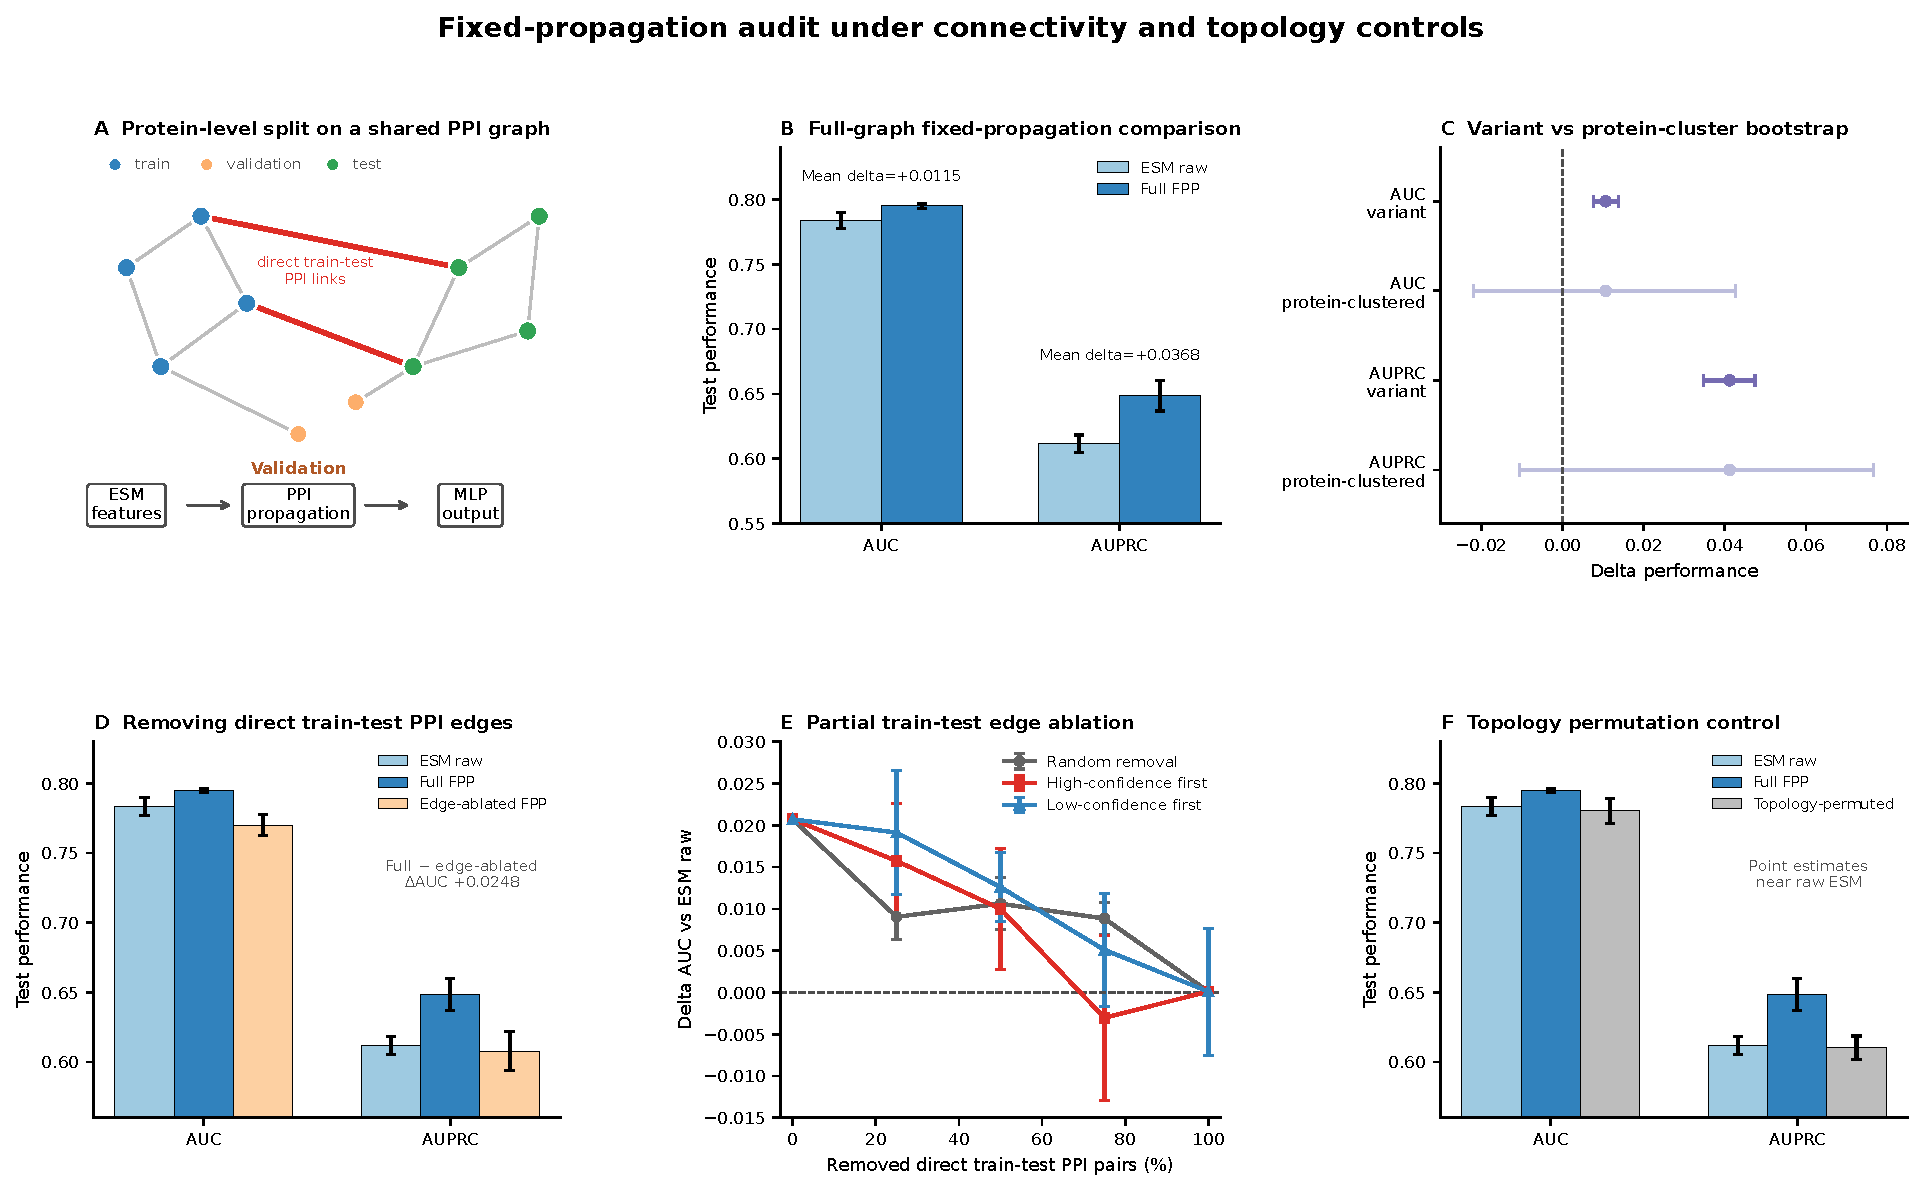
\includegraphics[width=0.98\textwidth]{figure_drafts/Figure1_connectivity_topology_controls_v2_accepted_minimal_clarified.pdf}
\caption{Fixed protein-feature propagation under connectivity and topology controls. A, ESM features are propagated over the STRING network before downstream MLP classification. B, Mean AUC and AUPRC for raw ESM and full FPP under matched classifier seeds; error bars denote sample standard deviation. C, Paired ensemble differences under variant-level and protein-clustered bootstrap resampling. D, Matched comparison of raw ESM, full FPP and direct-edge-ablated FPP. E, Partial train-test edge-ablation sensitivity analysis using a separate training protocol with reused endpoint estimates; implementation details are provided in Supplementary Table 8. F, Topology-permutation control using three graph permutations and three classifier seeds per graph. Bootstrap intervals are conditional on fitted models and the evaluated graphs.}
\label{fig:connectivity}
\end{figure*}

\subsection{Strong predictors and homology-aware evaluation bound PPI context gains}

Under the original split, single-score CADD and AlphaMissense baselines achieved AUC 0.9207 and 0.9470, respectively. The architecture-matched CADD+AlphaMissense baseline achieved mean AUC 0.9572 and AUPRC 0.9072. Adding raw ESM, edge-ablated FPP, topology-permuted FPP and full FPP yielded mean AUCs of 0.9682, 0.9704, 0.9692 and 0.9716, respectively (Fig. 2B; Supplementary Table 11). On averaged ensemble predictions, full FPP fusion improved over the score baseline by $\Delta$AUC +0.0147 (protein-clustered 95\% CI [+0.0065, +0.0226]) and over raw-ESM fusion by +0.0032 ([+0.0008, +0.0062]). Its margins over edge-ablated fusion (+0.0013, [$-$0.0004, +0.0032]) and topology-permuted fusion (+0.0020, [+0.0001, +0.0045]) were smaller (Fig. 2C; Supplementary Table 12). These results indicate substantial complementarity from protein representations, with a more limited additional contribution from the original STRING topology.

Under the homology-aware split, a separate single-fit representation comparison yielded AUC 0.7248 for raw ESM and 0.7606 for full FPP (Fig. 2D). In the matched three-seed fusion comparison, the CADD+AlphaMissense baseline achieved mean AUC 0.9755 and AUPRC 0.8403, compared with 0.9727 and 0.8253 for raw-ESM fusion and 0.9752 and 0.8369 for full-FPP fusion (Fig. 2E; Supplementary Table 11). On ensemble predictions, full-FPP fusion exceeded raw-ESM fusion by $\Delta$AUC +0.0027 (protein-clustered 95\% CI [+0.0015, +0.0040]), but its difference from the strong score baseline was +0.0001 ([$-$0.0019, +0.0020]; Supplementary Table 12). Thus, graph fusion provided a positive increment over raw-embedding fusion without establishing a clear additional benefit over CADD+AlphaMissense under homology-aware splitting. The test-set positive rate differed between the original and homology-aware splits (31.95\% versus 10.56\%; Fig. 2F), limiting direct cross-split AUPRC comparison.

\begin{figure*}[!t]
\centering
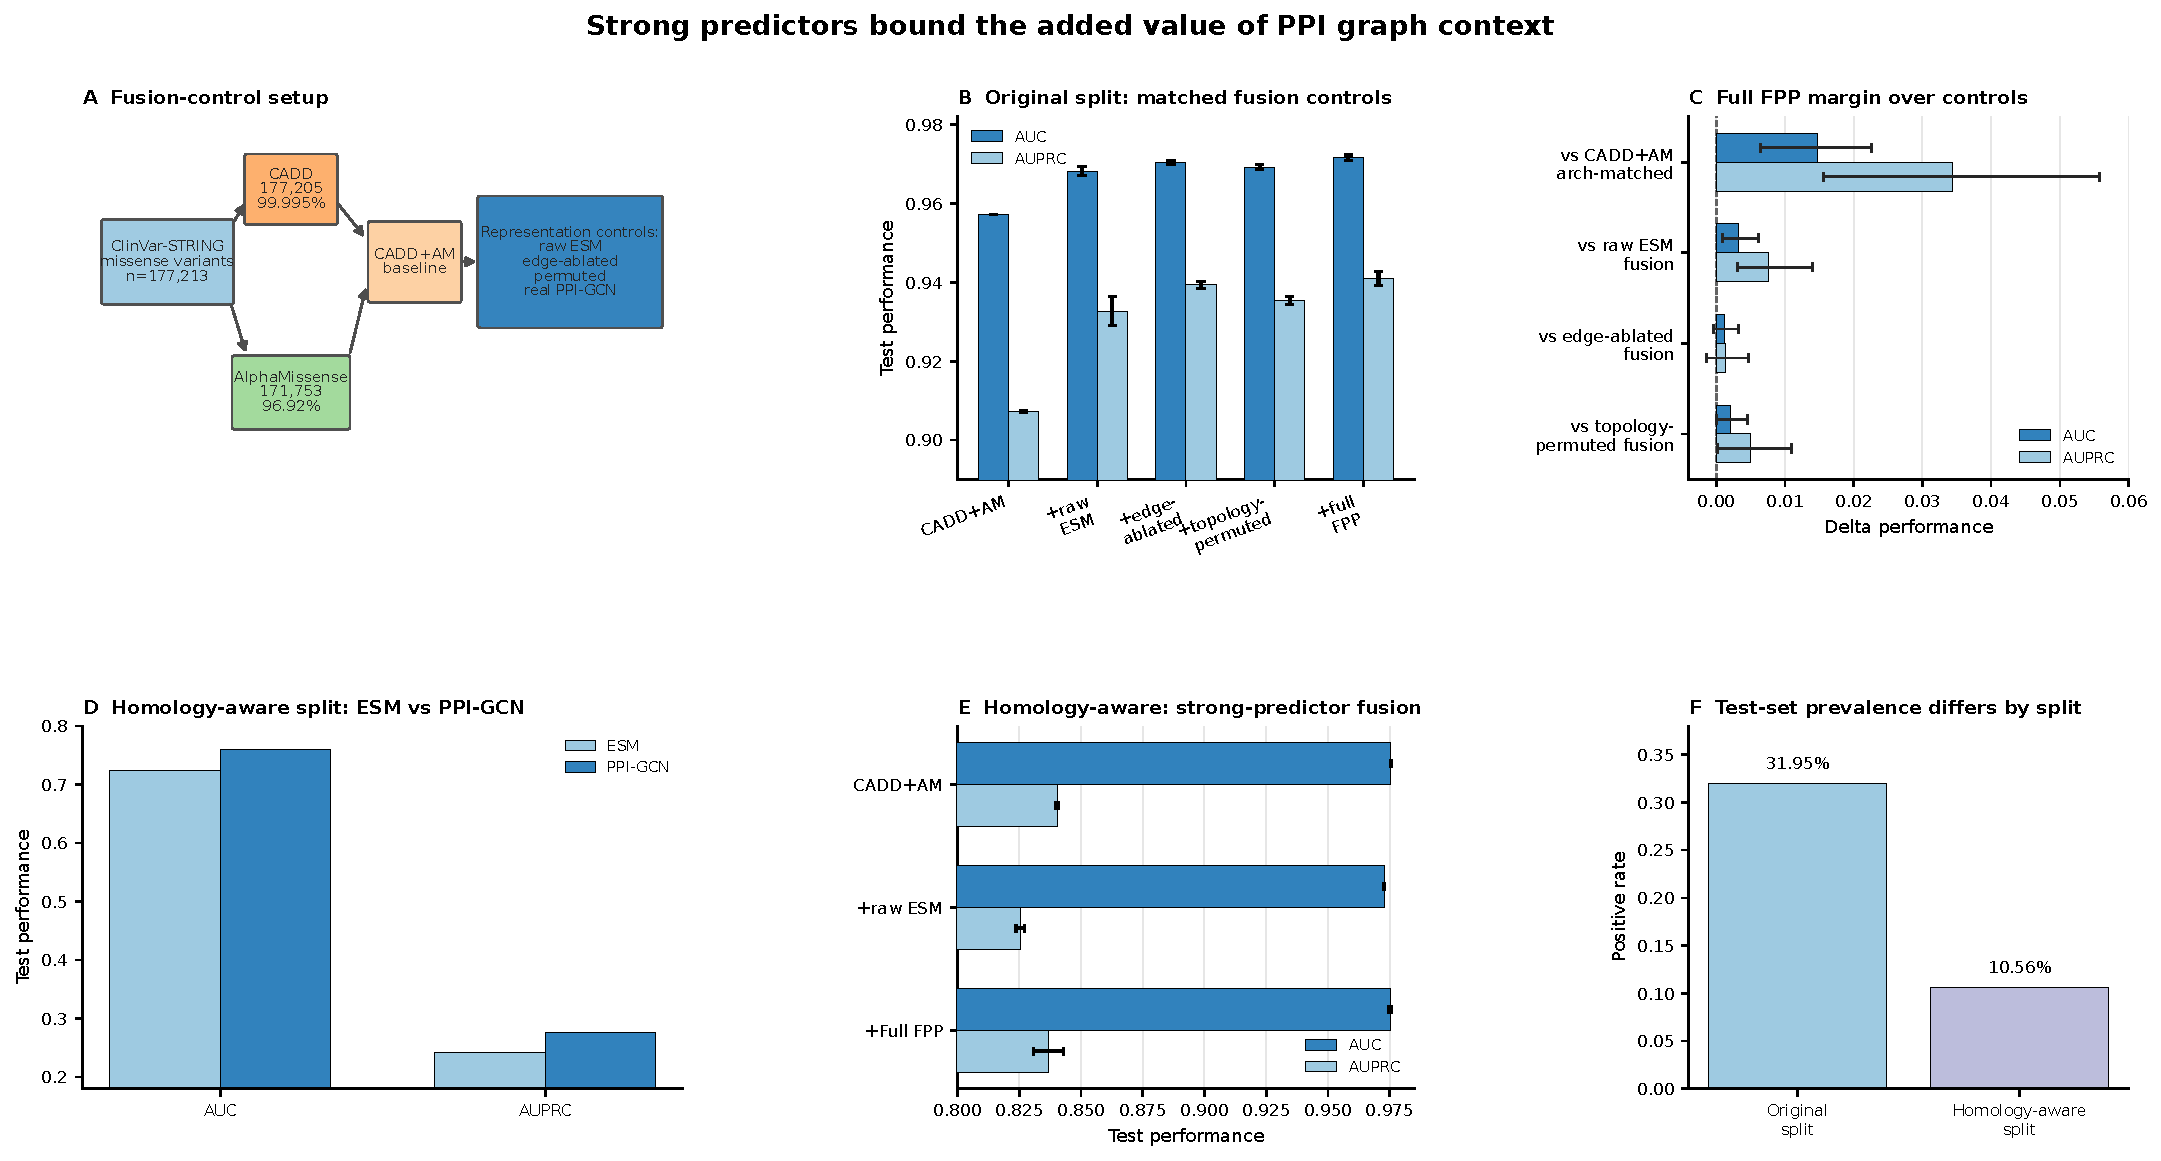
\includegraphics[width=0.98\textwidth]{figure_drafts/Figure2_fusion_homology_v1_accepted.pdf}
\caption{Strong-predictor fusion and homology-aware evaluation. A, Score coverage and fusion-control setup; architecture matching refers to the hidden-layer configuration, not equal input-layer parameter counts. B, Original-split fusion performance under matched training settings; error bars represent sample standard deviation across classifier fits. C, Full-FPP fusion differences relative to score-only and protein-representation controls, with paired protein-clustered bootstrap 95\% intervals computed from ensemble predictions. D, Single-fit comparison of raw ESM and full FPP representations under the homology-aware split. E, Three-seed matched fusion comparisons under the homology-aware split. F, Test-set positive prevalence for the original and homology-aware splits. Permutation controls use three graphs and three classifier seeds per graph.}
\label{fig:fusion_homology}
\end{figure*}

\subsection{Exploratory graph gains across topology contexts}

ESM protein representations showed modest correspondence with PPI topology. Directly connected protein pairs had a mean cosine similarity of 0.8789, compared with 0.8639 for randomly paired proteins; within-community similarity also exceeded between-community similarity (Fig. 3A). Performance differences between fixed PPI-GCN propagation and raw ESM varied non-monotonically across network strata. For example, mid-k-core variants showed a $\Delta$AUC of +0.0775, whereas high-degree variants showed $-$0.0178 (Fig. 3B). Betweenness, clustering and neighbour-risk strata also exhibited heterogeneous performance differences (Fig. 3C,D).

Among 53 joint topology cells examined on the same test set, we observed both positive and negative performance differences, including mid-k-core/high-betweenness ($\Delta$AUC +0.1429) and high-k-core/low-clustering ($\Delta$AUC $-$0.0532; Fig. 3E,F). Because the highlighted cells were selected after examining the test-set results and their intervals were computed using variant-level resampling, these estimates do not account for within-protein dependence or subgroup-selection uncertainty. We therefore interpret these patterns as exploratory findings that require independent validation.



\begin{figure*}[!t]
\centering
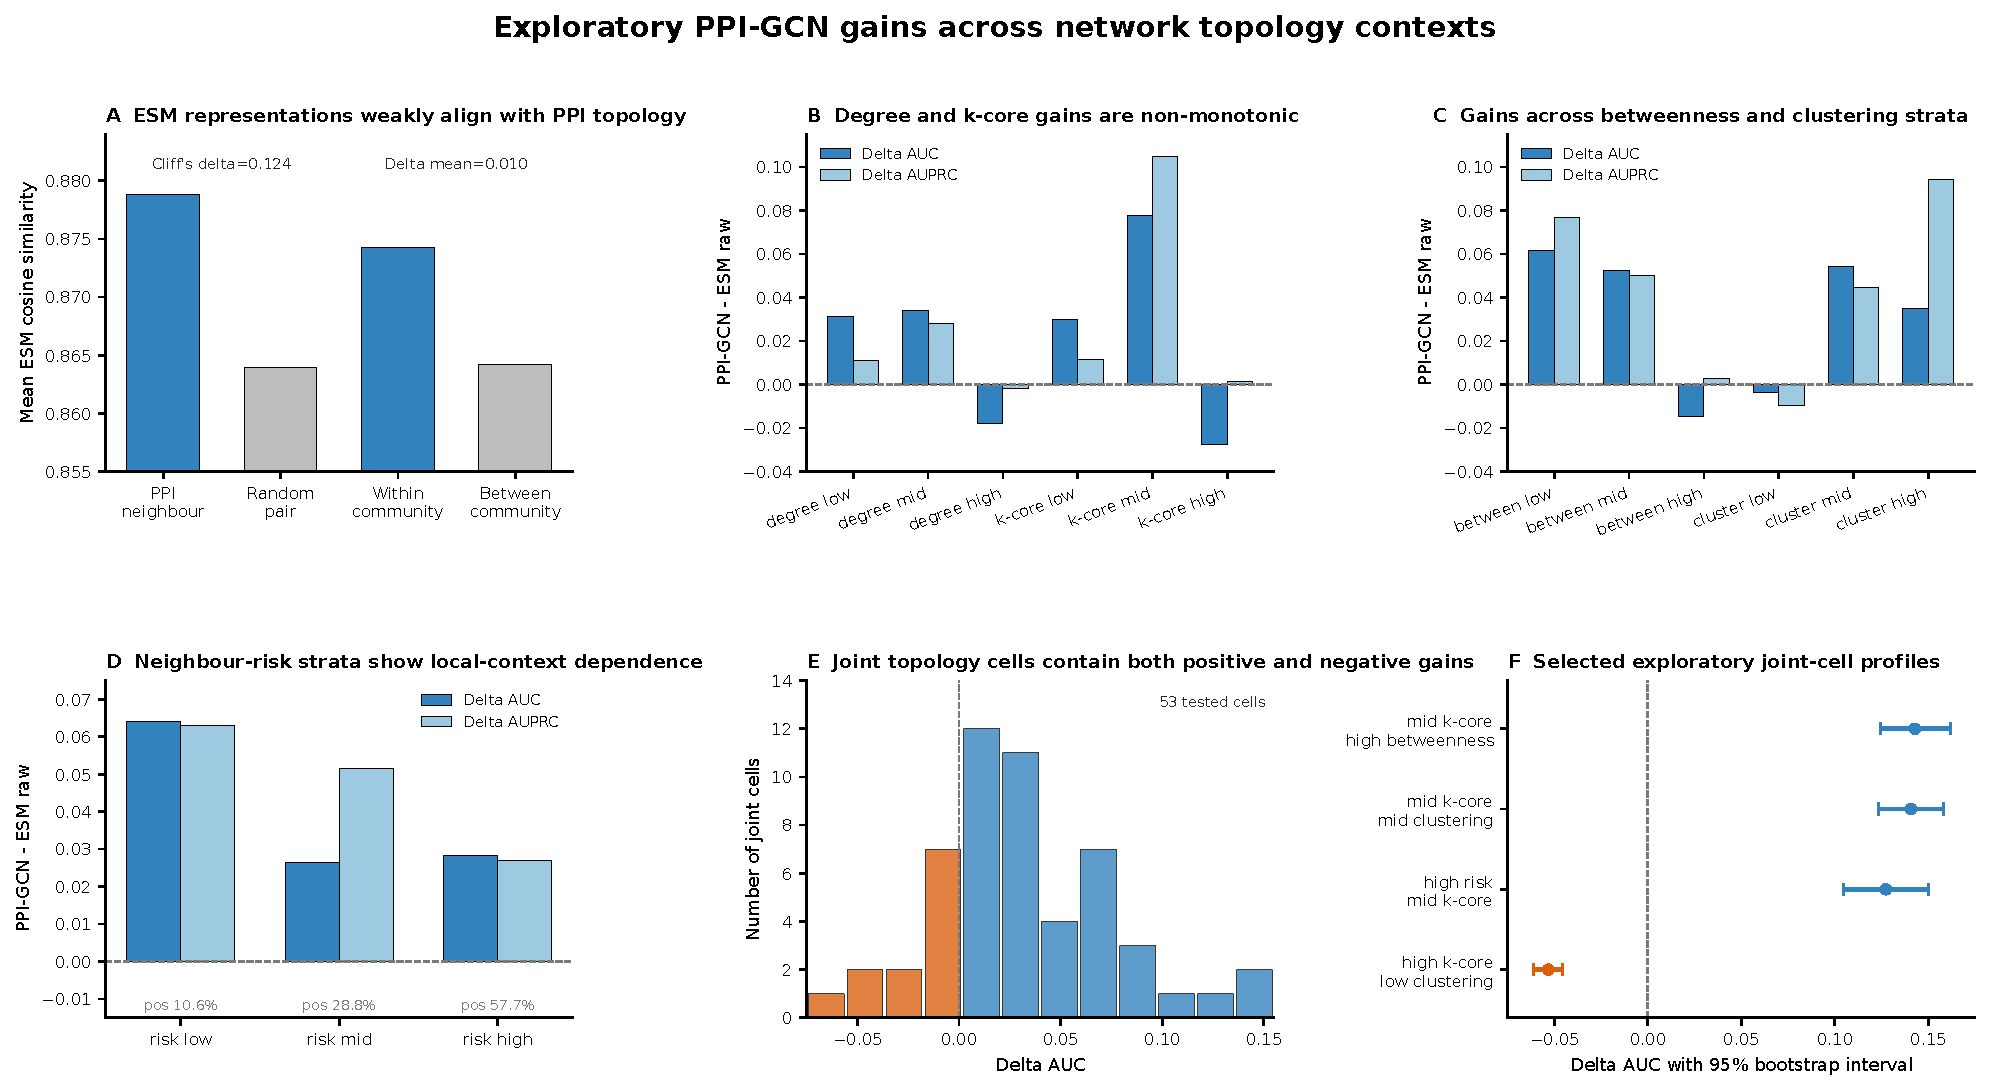
\includegraphics[width=0.98\textwidth]{figure_drafts/Figure3_topology_context_v1_accepted_clarified.pdf}
\caption{Exploratory topology-context analysis of fixed protein-feature propagation. A, ESM similarity across protein-network relationships. B--D, Performance differences between fixed PPI-GCN propagation and raw ESM across degree, k-core, betweenness, clustering and neighbour-risk strata. E, Distribution of AUC differences across 53 joint topology cells. F, Selected positive and negative joint-cell profiles with variant-level bootstrap intervals. Panels B--F use a fixed reference model pair. The selected profiles are descriptive, and their intervals do not account for within-protein dependence or post-hoc subgroup selection.}
\label{fig:topology_context}
\end{figure*}

\subsection{Graph augmentation reshapes false-negative and false-positive predictions differently}

At a threshold of 0.5, the three-seed raw-ESM and full-FPP ensembles were jointly correct for 12,520 test variants and jointly wrong for 3,747. Full FPP corrected 960 predictions and degraded 993: 366 false negatives were rescued and 594 false positives suppressed, while 958 true negatives became false positives and 35 true positives became false negatives (Fig. 4A). The net change was 33 additional classification errors at this threshold. Thus, the higher AUC and AUPRC point estimates did not translate into fewer classification errors at the fixed threshold of 0.5.

The architecture-matched \CADDAM{} and full-FPP fusion ensembles were jointly correct for 16,055 variants and jointly wrong for 1,262. Fusion corrected 679 predictions (170 rescued false negatives and 509 suppressed false positives) and degraded 224 (99 new false positives and 125 new false negatives), reducing the total errors by 455 (Fig. 4B).

Rescued false negatives had higher degree- and neighbour-risk-bucket means than suppressed false positives in both comparisons; their clustering coefficient was lower for the representation comparison and higher for fusion (Fig. 4C--E). Within raw-ESM baseline false negatives, rescued variants had higher degree-bucket means and within-community neighbour fractions than persistent false negatives (Hedges' \textit{g} +0.538 and +0.360; Fig. 4F). Repeated variants within proteins limit statistical inference, and these descriptive associations do not establish a mechanism.

\begin{figure*}[!p]
\centering
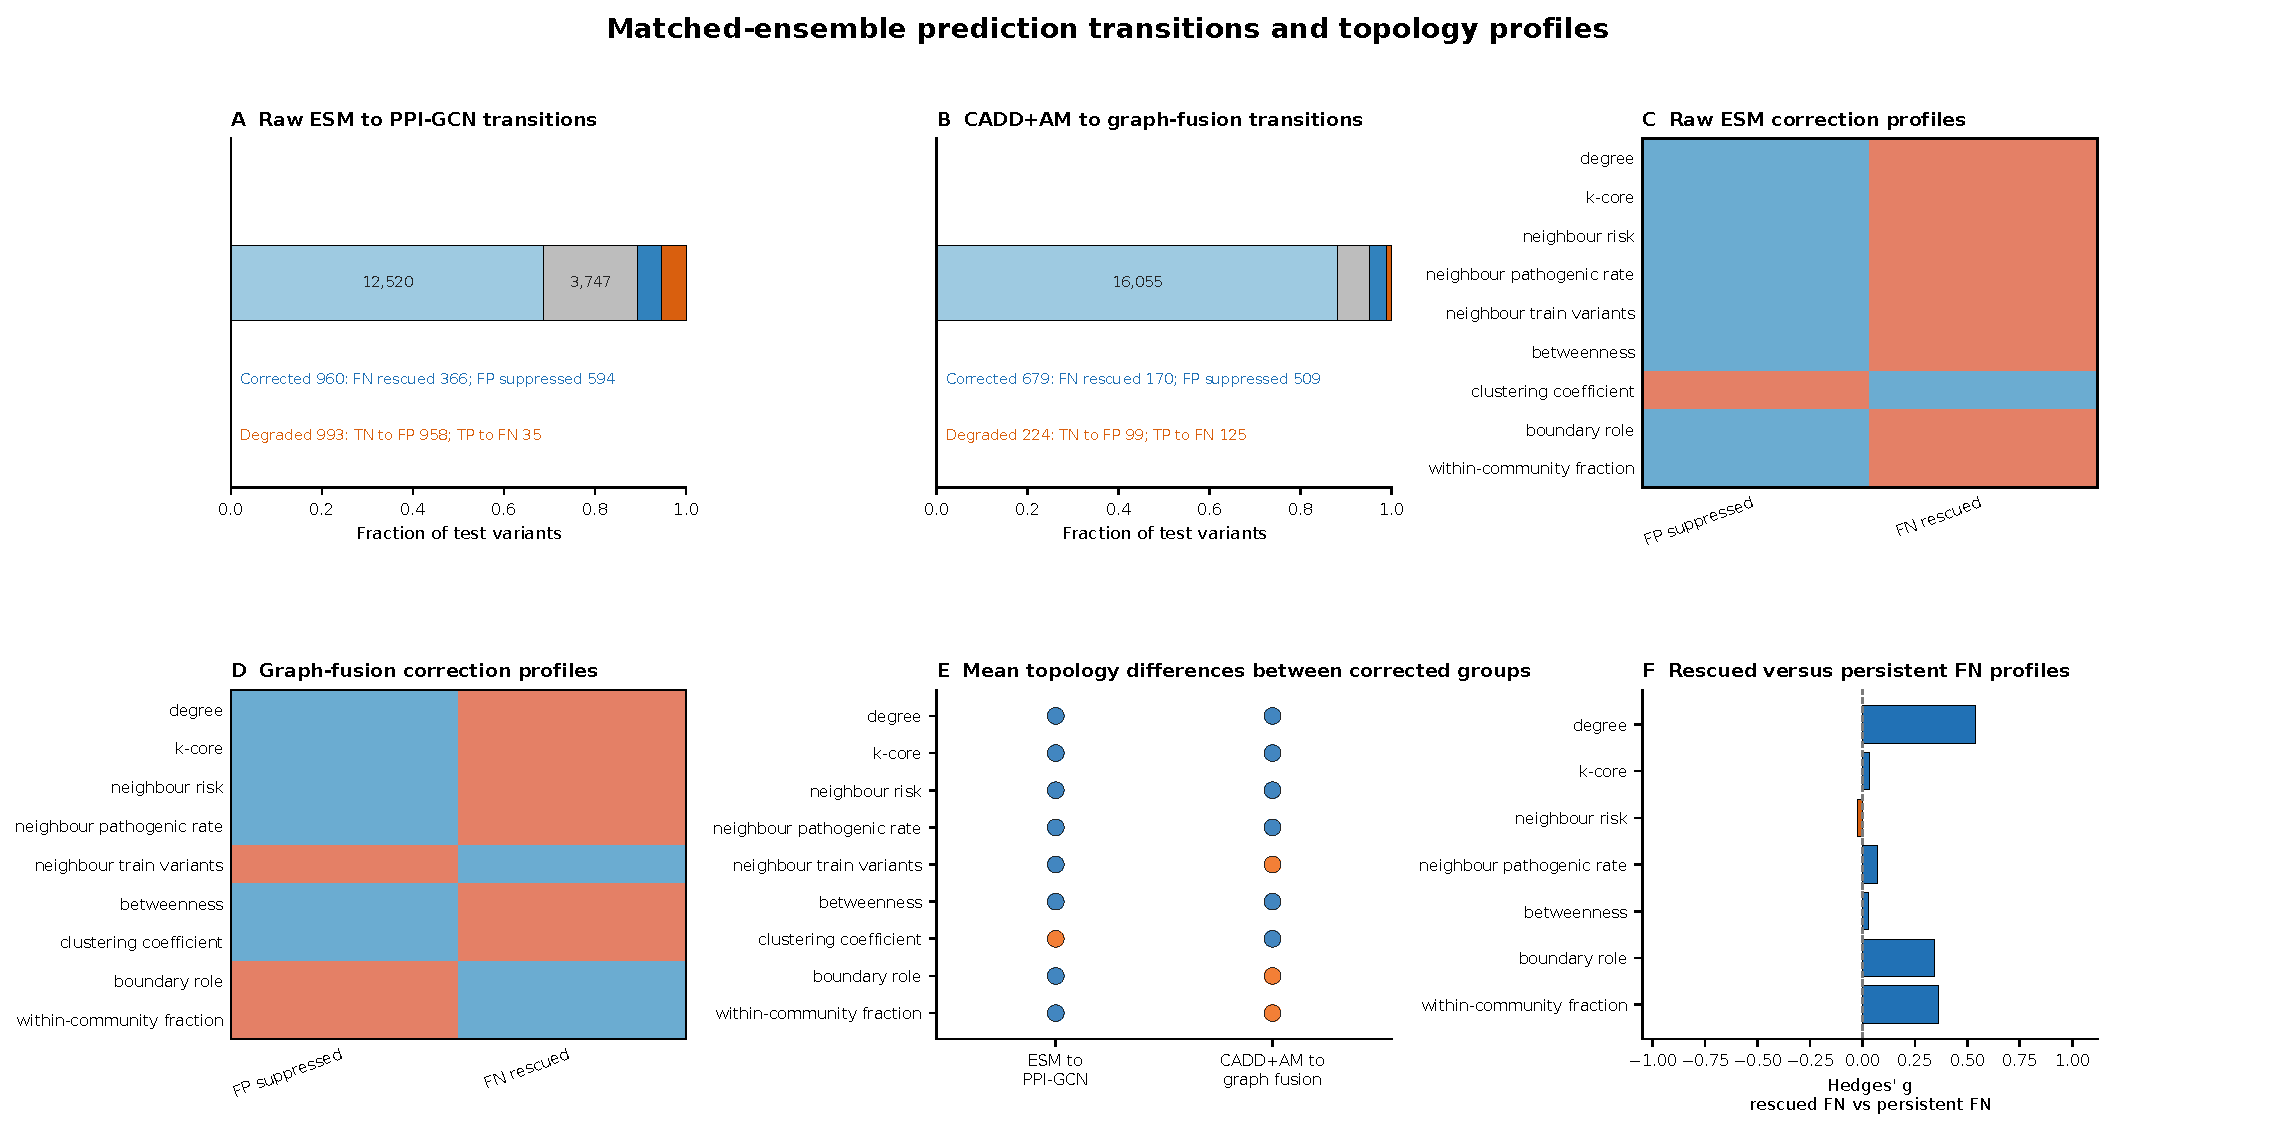
\includegraphics[width=0.98\textwidth]{figure_drafts/Figure4_prediction_transitions_matched_ensembles.pdf}
\caption{Prediction transitions and descriptive topology profiles from matched model ensembles. A--B, Prediction transitions at a threshold of 0.5 using mean probabilities across three classifier seeds per model: raw ESM versus full FPP (A), and CADD+AlphaMissense versus full-FPP fusion (B). C--D, Row-centered and range-scaled topology-feature means for rescued false negatives and suppressed false positives. E, Directional differences in feature means between the corrected groups. F, Descriptive Hedges' \textit{g} comparing false negatives rescued by full FPP with persistent false negatives within the raw-ESM baseline false-negative group. The topology-feature analyses are descriptive; repeated variants within proteins limit statistical inference. In C--D, warm/blue colors denote means above/below the within-row mean; color magnitudes are not comparable across features. In E, blue/orange denotes higher means among rescued false negatives/suppressed false positives; in F, blue/orange denotes positive/negative effects.}
\label{fig:prediction_transitions}
\end{figure*}


\subsection{External-source and second-network validation}

On the primary external set, mean AUC across three seeds was 0.6932 for raw ESM, 0.7304 for STRING propagation and 0.7025 for BioGRID. STRING-minus-raw ensemble gains were +0.0375 AUC (protein 95\% CI [+0.0173, +0.0564]) and +0.0463 AUPRC ([+0.0151, +0.0745]). The nested stricter subset supported the same AUC direction (+0.0352, [+0.0034, +0.0667]); BioGRID-versus-raw intervals crossed zero in both sets (Fig.~\ref{fig:external}A).

On the original split, BioGRID fusion improved over scores alone ($\Delta$AUC +0.0124, [+0.0034, +0.0210]), but its added benefit over raw-embedding fusion remained uncertain (+0.0009, [-0.0011, +0.0036]). BioGRID fusion was below STRING fusion under the fitted-ensemble intervals in both splits (Fig.~\ref{fig:external}B). External gains and fusion complementarity therefore depend on network choice and comparator.

\begin{figure*}[!p]
\centering
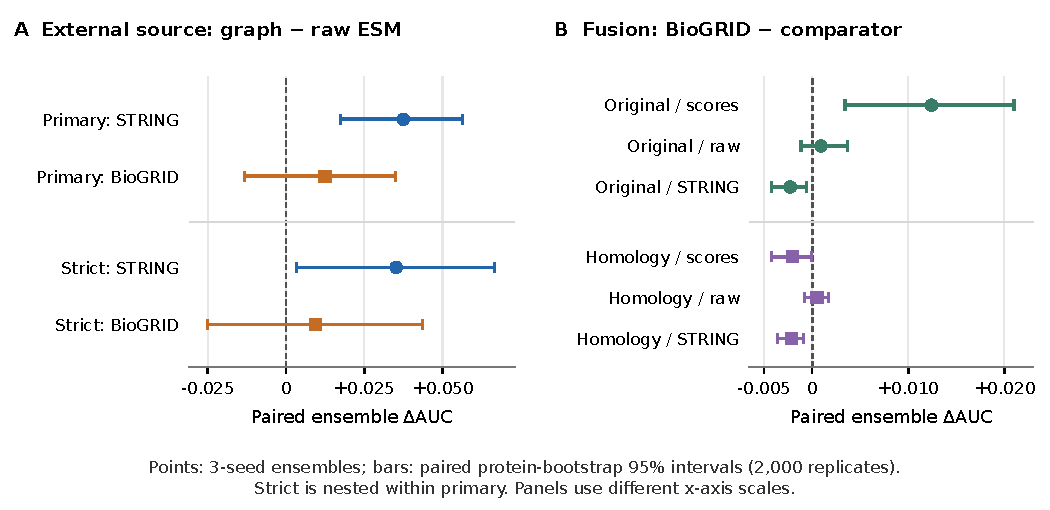
\includegraphics[width=0.98\textwidth]{figure_drafts/Figure5_external_validation.pdf}
\caption{Additional external-source and second-network validation. A, STRING/BioGRID propagation minus raw-ESM AUC on the primary HUMSAVAR set (10,785 variants; 2,498 proteins) and nested strict subset (6,934; 1,713). B, BioGRID fusion minus scores alone, raw-embedding fusion or STRING fusion in each split. Points use three-seed mean probabilities; bars are paired protein-bootstrap 95\% intervals (2,000 resamples), conditional on fitted models. Intervals are exploratory without multiplicity adjustment. All evaluated proteins remain frozen-graph nodes; the strict set is nested, not a second replication.}
\label{fig:external}
\end{figure*}

\section{Discussion}

Under the original protein-level split, full FPP achieved higher mean AUC and AUPRC than raw ESM, although the protein-clustered confidence interval for the ensemble AUC gain included zero. Removing direct train-test connections reduced performance under matched training settings, indicating connectivity sensitivity without isolating the effect of direct edges from changes in graph normalization. With CADD+AlphaMissense included, much of the fusion improvement was also observed after adding raw ESM, while full FPP provided a smaller additional increment over raw-ESM fusion (ensemble $\Delta$AUC +0.0032, 95\% CI [+0.0008, +0.0062]). These findings support protein-representation complementarity, with a limited additional contribution from STRING graph context under the original split.

Under the homology-aware split, full-FPP fusion improved over raw-ESM fusion (ensemble $\Delta$AUC +0.0027, protein-clustered 95\% CI [+0.0015, +0.0040]) but did not establish a clear advantage over the architecture-matched CADD+AlphaMissense baseline ($\Delta$AUC +0.0001, 95\% CI [$-$0.0019, +0.0020]). Redundant high-dimensional features, additional input-layer parameters, overfitting, feature scaling and differences in protein composition may contribute to the limited incremental benefit; these explanations were not tested individually. The difference in test-set positive prevalence also limits direct AUPRC comparisons between the original and homology-aware splits.

The matched ensembles showed different error trade-offs at the same decision threshold. At 0.5, full FPP produced 33 more classification errors than raw ESM despite higher AUC and AUPRC point estimates, whereas full-FPP fusion produced 455 fewer errors than the score-only baseline (Fig. 4A,B). Ranking improvements therefore did not uniformly translate into fewer threshold-specific errors. The topology profiles describe differences between error-transition groups rather than established correction mechanisms. External HUMSAVAR evaluation supports transfer of STRING-based representations under the specified exclusions, while BioGRID's external gains over raw ESM and incremental fusion gains over raw-embedding fusion remained uncertain. HUMSAVAR and ClinVar may share annotation evidence, and STRING and BioGRID overlap; these comparisons do not constitute independent-patient or prospective validation.

The evaluation has several constraints. ClinVar labels may reflect submission bias and future updates \cite{Landrum2020ClinVar}. Unknown development-data overlap for CADD and AlphaMissense limits prospective interpretation. Protein-level mapping omits isoform and residue-specific effects. STRING associations extend beyond direct physical interactions \cite{Szklarczyk2023STRING}; transductive propagation and direct-edge ablation retain indirect cross-partition paths. Outputs from class-weighted training are not calibrated clinical probabilities, and transition counts depend on the chosen threshold. The external set excludes specified variants/proteins but not all homologues or shared annotation evidence; external clinical-score fusion was not evaluated. These findings concern fixed propagation and should not be generalized to trained graph neural networks.

\noindent\textit{Practical recommendations:}
Compare graph features with raw embeddings and strong score baselines under matched training settings. State whether held-out proteins remain visible in the graph, assess uncertainty at the protein level, and treat selected topology groups as hypotheses. Check calibration and decision thresholds before clinical use.

\section*{Data and Code Availability}

Supplementary Information, code, compact source data, complete sample memberships, per-seed predictions, protocols and checksums are publicly available at \url{https://github.com/brynn-t02/ppi-graph-missense-audit}. Large provider resources, feature tensors and model checkpoints are stored separately; third-party source data should be obtained from their original providers.

\section*{Acknowledgment}

OpenAI ChatGPT, OpenAI Codex and Anthropic Claude assisted with literature organization, code development, manuscript language editing, and scripts for environment restoration, model fitting. We take responsibility for study design, experimental execution and verification, code review, result interpretation, reference checking and the final manuscript.

\begin{thebibliography}{99}
\bibitem{Kircher2014CADD} M. Kircher et al., ``A general framework for estimating the relative pathogenicity of human genetic variants,'' \emph{Nature Genetics}, vol. 46, pp. 310--315, 2014, doi: 10.1038/ng.2892.
\bibitem{Ioannidis2016REVEL} N. M. Ioannidis et al., ``REVEL: an ensemble method for predicting the pathogenicity of rare missense variants,'' \emph{American Journal of Human Genetics}, vol. 99, pp. 877--885, 2016, doi: 10.1016/j.ajhg.2016.08.016.
\bibitem{Qi2021MVP} H. Qi et al., ``MVP predicts the pathogenicity of missense variants by deep learning,'' \emph{Nature Communications}, vol. 12, p. 510, 2021, doi: 10.1038/s41467-020-20847-0.
\bibitem{Sundaram2018PrimateAI} L. Sundaram et al., ``Predicting the clinical impact of human mutation with deep neural networks,'' \emph{Nature Genetics}, vol. 50, pp. 1161--1170, 2018, doi: 10.1038/s41588-018-0167-z.
\bibitem{Frazer2021EVE} J. Frazer et al., ``Disease variant prediction with deep generative models of evolutionary data,'' \emph{Nature}, vol. 599, pp. 91--95, 2021, doi: 10.1038/s41586-021-04043-8.
\bibitem{Cheng2023AlphaMissense} J. Cheng et al., ``Accurate proteome-wide missense variant effect prediction with AlphaMissense,'' \emph{Science}, vol. 381, eadg7492, 2023, doi: 10.1126/science.adg7492.
\bibitem{Lin2023ESM} Z. Lin et al., ``Evolutionary-scale prediction of atomic-level protein structure with a language model,'' \emph{Science}, vol. 379, pp. 1123--1130, 2023, doi: 10.1126/science.ade2574.
\bibitem{Barabasi2011NetworkMedicine} A.-L. Barabasi, N. Gulbahce, and J. Loscalzo, ``Network medicine: a network-based approach to human disease,'' \emph{Nature Reviews Genetics}, vol. 12, pp. 56--68, 2011, doi: 10.1038/nrg2918.
\bibitem{Menche2015DiseaseModules} J. Menche et al., ``Disease networks. Uncovering disease-disease relationships through the incomplete interactome,'' \emph{Science}, vol. 347, 1257601, 2015, doi: 10.1126/science.1257601.
\bibitem{Sahni2015InteractionPerturbation} N. Sahni et al., ``Widespread macromolecular interaction perturbations in human genetic disorders,'' \emph{Cell}, vol. 161, pp. 647--660, 2015, doi: 10.1016/j.cell.2015.04.013.
\bibitem{Chen2018InteractomePerturbation} S. Chen et al., ``An interactome perturbation framework prioritizes damaging missense mutations for developmental disorders,'' \emph{Nature Genetics}, vol. 50, pp. 1032--1040, 2018, doi: 10.1038/s41588-018-0130-z.
\bibitem{Yates2014SuSPect} C. M. Yates, I. Filippis, L. A. Kelley, and M. J. E. Sternberg, ``SuSPect: enhanced prediction of single amino acid variant (SAV) phenotype using network features,'' \emph{Journal of Molecular Biology}, vol. 426, pp. 2692--2701, 2014, doi: 10.1016/j.jmb.2014.04.026.
\bibitem{Ozturk2022NetworkFeatures} K. Ozturk and H. Carter, ``Predicting functional consequences of mutations using molecular interaction network features,'' \emph{Human Genetics}, vol. 141, pp. 1195--1210, 2022, doi: 10.1007/s00439-021-02329-5.
\bibitem{Zhang2022gMVP} H. Zhang, M. S. Xu, X. Fan, W. K. Chung, and Y. Shen, ``Predicting functional effect of missense variants using graph attention neural networks,'' \emph{Nature Machine Intelligence}, vol. 4, no. 11, pp. 1017--1028, 2022, doi: 10.1038/s42256-022-00561-w.
\bibitem{Cheng2021VEGN} J. Cheng, C. Lawrence, and M. Niepert, ``VEGN: variant effect prediction with graph neural networks,'' arXiv:2106.13642, 2021, doi: 10.48550/arXiv.2106.13642.
\bibitem{Yu2025GNNMAP} H. Yu et al., ``A graph neural network approach for accurate prediction of pathogenicity in multi-type variants,'' \emph{Briefings in Bioinformatics}, vol. 26, bbaf151, 2025, doi: 10.1093/bib/bbaf151.
\bibitem{Ghadie2025DiseaseSpecificGNN} M. Ghadie, S. Sardaar, and Y. Trakadis, ``Disease-specific prediction of missense variant pathogenicity with DNA language models and graph neural networks,'' \emph{Bioengineering}, vol. 12, p. 1098, 2025, doi: 10.3390/bioengineering12101098.
\bibitem{Littmann2022ProteinMLTips} Q. Hou, K. Waury, D. Gogishvili, and K. A. Feenstra, ``Ten quick tips for sequence-based prediction of protein properties using machine learning,'' \emph{PLOS Computational Biology}, vol. 18, no. 12, Art. no. e1010669, 2022, doi: 10.1371/journal.pcbi.1010669.
\bibitem{Teufel2023GraphPart} F. Teufel, M. H. Gislason, J. J. Almagro Armenteros, A. R. Johansen, O. Winther, and H. Nielsen, ``GraphPart: homology partitioning for biological sequence analysis,'' \emph{NAR Genomics and Bioinformatics}, vol. 5, lqad088, 2023, doi: 10.1093/nargab/lqad088.
\bibitem{Landrum2020ClinVar} M. J. Landrum et al., ``ClinVar: improvements to accessing data,'' \emph{Nucleic Acids Research}, vol. 48, pp. D835--D844, 2020, doi: 10.1093/nar/gkz972.
\bibitem{Szklarczyk2023STRING} D. Szklarczyk et al., ``The STRING database in 2023: protein-protein association networks and functional enrichment analyses for any sequenced genome of interest,'' \emph{Nucleic Acids Research}, vol. 51, pp. D638--D646, 2023, doi: 10.1093/nar/gkac1000.
\bibitem{Kipf2017GCN} T. N. Kipf and M. Welling, ``Semi-supervised classification with graph convolutional networks,'' \emph{International Conference on Learning Representations}, 2017.
\bibitem{Steinegger2017MMseqs2} M. Steinegger and J. Soding, ``MMseqs2 enables sensitive protein sequence searching for the analysis of massive data sets,'' \emph{Nature Biotechnology}, vol. 35, pp. 1026--1028, 2017, doi: 10.1038/nbt.3988.
\bibitem{Kingma2015Adam} D. P. Kingma and J. Ba, ``Adam: a method for stochastic optimization,'' \emph{International Conference on Learning Representations}, 2015, arXiv:1412.6980.
\bibitem{Schubach2024CADDv17} M. Schubach et al., ``CADD v1.7: using protein language models, regulatory CNNs and other nucleotide-level scores to improve genome-wide variant predictions,'' \emph{Nucleic Acids Research}, vol. 52, no. D1, pp. D1143--D1154, 2024, doi: 10.1093/nar/gkad989.
\bibitem{Efron1993Bootstrap} B. Efron and R. J. Tibshirani, \emph{An Introduction to the Bootstrap}. Chapman \& Hall/CRC, 1993.
\bibitem{Benjamini1995FDR} Y. Benjamini and Y. Hochberg, ``Controlling the false discovery rate: a practical and powerful approach to multiple testing,'' \emph{Journal of the Royal Statistical Society: Series B}, vol. 57, pp. 289--300, 1995, doi: 10.1111/j.2517-6161.1995.tb02031.x.
\bibitem{Saito2015PrecisionRecall} T. Saito and M. Rehmsmeier, ``The precision-recall plot is more informative than the ROC plot when evaluating binary classifiers on imbalanced datasets,'' \emph{PLOS ONE}, vol. 10, e0118432, 2015, doi: 10.1371/journal.pone.0118432.
\bibitem{UniProt2025} The UniProt Consortium, ``UniProt: the Universal Protein Knowledgebase in 2025,'' \emph{Nucleic Acids Research}, vol. 53, no. D1, pp. D609--D617, 2025, doi: 10.1093/nar/gkae1010.
\bibitem{Stark2006BioGRID} C. Stark, B.-J. Breitkreutz, T. Reguly, L. Boucher, A. Breitkreutz, and M. Tyers, ``BioGRID: a general repository for interaction datasets,'' \emph{Nucleic Acids Research}, vol. 34, pp. D535--D539, 2006, doi: 10.1093/nar/gkj109.
\end{thebibliography}
\end{document}
